% ======================================================================
% TASK プラズマ輸送ライブラリ化プロジェクト マニュアル (日本語)
%
% Build:
%   xelatex -interaction=nonstopmode task-library-manual.tex
%   xelatex -interaction=nonstopmode task-library-manual.tex
%
% Fonts: Noto Serif CJK JP / Noto Sans CJK JP / Noto Sans Mono CJK JP
% ======================================================================
\documentclass[11pt,a4paper]{report}
\usepackage[margin=2.5cm]{geometry}
\usepackage{xeCJK}
\usepackage{fontspec}
\setCJKmainfont{Noto Serif CJK JP}
\setCJKsansfont{Noto Sans CJK JP}
\setCJKmonofont{Noto Sans Mono CJK JP}
\setmonofont{DejaVu Sans Mono}
\usepackage{listings,xcolor,longtable,booktabs,hyperref,fancyhdr}
\usepackage{tcolorbox}
\tcbuselibrary{breakable,skins}
\usepackage{tikz}
\usetikzlibrary{positioning,arrows.meta,shapes.geometric,fit,calc,backgrounds}
\usepackage{enumitem,graphicx,array,caption}
\hypersetup{colorlinks=true,linkcolor=blue,urlcolor=magenta,bookmarksopen=true}

% ---- Custom tcolorboxes ------------------------------------------------
\newtcolorbox{faq}[1][]{%
  colback=yellow!8,colframe=orange!75!black,title=#1,
  fonttitle=\bfseries,breakable}
\newtcolorbox{learn}[1][この章で学ぶこと]{%
  colback=blue!5,colframe=blue!60!black,title=#1,
  fonttitle=\bfseries,breakable}
\newtcolorbox{note}[1][補足]{%
  colback=gray!6,colframe=gray!60!black,title=#1,
  fonttitle=\bfseries,breakable}
\newtcolorbox{warn}[1][注意]{%
  colback=red!5,colframe=red!60!black,title=#1,
  fonttitle=\bfseries,breakable}

% ---- Listing styles ----------------------------------------------------
\definecolor{kwblue}{RGB}{0,64,192}
\definecolor{cmgreen}{RGB}{0,120,0}
\definecolor{strpurple}{RGB}{128,0,128}
\definecolor{bggray}{RGB}{248,248,248}

\lstdefinestyle{base}{%
  backgroundcolor=\color{bggray},
  basicstyle=\ttfamily\footnotesize,
  keywordstyle=\color{kwblue}\bfseries,
  commentstyle=\color{cmgreen}\itshape,
  stringstyle=\color{strpurple},
  numbers=left,numberstyle=\tiny\color{gray},
  numbersep=8pt,
  frame=single,framesep=4pt,
  showstringspaces=false,
  breaklines=true,
  breakatwhitespace=false,
  columns=fullflexible,
  keepspaces=true,
  tabsize=2}

\lstdefinestyle{py}{style=base,language=Python}
\lstdefinestyle{bash}{style=base,language=bash}
\lstdefinestyle{c}{style=base,language=C}
\lstdefinestyle{fortran}{style=base,language=[90]Fortran,
  morekeywords={USE,ONLY,IMPLICIT,NONE,MODULE,PRIVATE,PUBLIC,CONTAINS,
                FUNCTION,SUBROUTINE,INTEGER,REAL,CHARACTER,INTENT,IN,OUT,
                RESULT,SELECT,CASE,DEFAULT,IF,THEN,ELSE,END,RETURN}}
\lstdefinestyle{plain}{style=base,language=}
\lstset{style=plain}

% ---- Header / Footer ---------------------------------------------------
\pagestyle{fancy}
\fancyhf{}
\fancyhead[L]{\small TASK プラズマ輸送ライブラリ化 — 日本語マニュアル}
\fancyhead[R]{\small \leftmark}
\fancyfoot[C]{\thepage}
\renewcommand{\headrulewidth}{0.4pt}

% ---- Metadata ----------------------------------------------------------
\title{\Huge TASK プラズマ輸送ライブラリ化プロジェクト\\
       \Large 日本語マニュアル・報告書 \\
       \large (tr / ti / wr / wrx / fp モジュール, Phase L-0 〜 L-7)}
\author{k-yoshimi (東京大学)}
\date{2026 年 4 月 18 日}

\begin{document}
\maketitle

\begin{abstract}\noindent
本書は TASK コード群 (プラズマ統合輸送シミュレーション) のうち,
5 つの物理モジュール---\textbf{tr} (1 次元輸送), \textbf{ti} (不純物
輸送), \textbf{wr} (波動レイトレーシング), \textbf{wrx} (拡張レイ
トレーシング), \textbf{fp} (Fokker--Planck 解析)---を \emph{共有
ライブラリ化} し, \emph{Python から利用可能} にした一連の作業
(Phase L-0 〜 L-7) を, Fortran や ctypes に馴染みのない初学者にも
読めるようにまとめたマニュアルである.

使い方章 (第 3〜7 章) は\textbf{です・ます調}で平易に記述し, 技術章
(第 8〜10 章) は\textbf{だ・である調}で手短にまとめる.
\end{abstract}

\tableofcontents
\clearpage

% ======================================================================
\chapter{はじめに}
\label{ch:intro}

\begin{learn}
本章では, 本書が何であるかと, 読者がどんな力を得られるかを整理します.
ここは読み飛ばさずに目を通しておくと, 後の章で迷子になりにくくなります.
\end{learn}

\section{本書の目的}

TASK コード群 (京都大学・東京大学で長年開発されているプラズマ統合
シミュレーションコード) の一部モジュールが, 2026 年 4 月の集中開発で
「共有ライブラリ (\texttt{.so} ファイル)」として配布・利用できるように
なりました. これによって,

\begin{itemize}[leftmargin=1.5em]
  \item Fortran の \texttt{tr2} や \texttt{fp} といった対話型プログラムを
        起動しなくても,
  \item Python スクリプトから\textbf{関数呼び出し感覚}で
        プラズマ輸送計算を回せる,
\end{itemize}

ようになりました.

本書はその\textbf{使い方}と\textbf{作業内容}を記録するマニュアル兼
報告書です.

\section{読者対象 (いちばん大事なところ)}

次のような方を想定しています.

\begin{itemize}[leftmargin=1.5em]
  \item プラズマ物理に興味がある学生, ただし Fortran は書いたことがない
  \item Python は少し触ったが, \texttt{ctypes} や共有ライブラリは聞いたこと
        がない
  \item ターミナルで \texttt{cd}, \texttt{ls}, \texttt{make} くらいは
        使える
\end{itemize}

「C, Fortran, 共有ライブラリ」などの用語は\textbf{最初に出てきた場所で
毎回説明します}. 分からない用語が出てきたら, 近くの\fbox{補足}や
\fbox{FAQ} を確認してください.

\section{本書で何ができるようになるか}

読み終えたときに, 次のことが自分の手で出来るようになります.

\begin{enumerate}[leftmargin=1.5em]
  \item TASK のソースから \texttt{libtrapi.so} などの共有ライブラリを
        ビルドする
  \item Python スクリプト 5 行で tr / ti / wr / wrx / fp のいずれかの
        計算を回し, 結果を dict として受け取る
  \item パラメータ名と値を指定してパラメータスキャンループを書く
  \item 4 層の回帰テスト (\texttt{run\_tests.sh}) で自分の変更が
        Phase 0 ベースラインと 1e-10 で一致することを確認する
\end{enumerate}

\section{前提ソフトウェア}

\begin{itemize}[leftmargin=1.5em]
  \item GNU/Linux (Ubuntu 22.04 以降で検証) もしくは同等 Unix
  \item gfortran 9 以降, gcc 9 以降, GNU Make
  \item Python 3.8 以降 (標準ライブラリのみで動作. NumPy は任意)
  \item Git
\end{itemize}

詳細な OS パッケージは \texttt{INSTALL\_Ubuntu.md} を参照してください.

\section{本書の構成}

\begin{itemize}[leftmargin=1.5em]
  \item 第 \ref{ch:arch} 章 — 全モジュール共通の構造. TikZ 3 層図と
        5 関数 API の説明.
  \item 第 \ref{ch:tr} 〜 \ref{ch:fp} 章 — tr / ti / wr / wrx / fp の
        各モジュール. 初学者向け hello-world と FAQ を含む.
  \item 第 \ref{ch:tests} 章 — 4 層テスト基盤.
  \item 第 \ref{ch:status} 章 — 作業状況 (完了/未完了, eq/tot 除外理由).
  \item 第 \ref{ch:appendix} 章 — 付録 (Makefile ターゲット, PR 一覧,
        参考資料).
\end{itemize}

\section{表記規約}

\begin{itemize}[leftmargin=1.5em]
  \item \texttt{\$} はシェルのプロンプトです. \texttt{\$} の後ろを
        ターミナルに打ち込んでください.
  \item \texttt{>>>} は Python の対話プロンプトです.
  \item コード中の日本語コメントは, あえて全角で書くことで実際の
        挙動と区別しています. 実コードには入れないでください.
\end{itemize}

% ======================================================================
\chapter{共通アーキテクチャ}
\label{ch:arch}

\begin{learn}
本章では, tr / ti / wr / wrx / fp のすべてに共通する 3 層構造,
5 関数 C ABI, エラーコード 0〜4, PIC ビルド, Python ctypes の
2 層設計を学びます. 以降の章はすべてこの章の応用です.
\end{learn}

\section{全体像 — 3 層アーキテクチャ}

すべての \texttt{X}lib (X は tr / ti / wr / wrx / fp のどれか) は
同じ 3 層構造を持ちます.

\vspace{1em}
\begin{center}
\begin{tikzpicture}[node distance=1.6cm,
      layer/.style={rectangle,draw,rounded corners,minimum width=11cm,
                    minimum height=1.3cm,align=center,font=\small},
      arr/.style={-{Latex[length=3mm]},thick}]
  \node[layer,fill=blue!15]  (u) {\textbf{ユーザ層} (Python スクリプト / C ドライバ / Jupyter Notebook)};
  \node[layer,fill=green!15,below=of u] (p) {\textbf{Python ラッパ層}\\
        \texttt{python/Xlib/}: \texttt{Xlib} クラス, \texttt{XState} dataclass, 例外階層, \texttt{\_ffi.py} (ctypes)};
  \node[layer,fill=yellow!20,below=of p] (c) {\textbf{C ABI 層} (5 関数 + 2 構造体)\\
        \texttt{X/X\_api.h}: \texttt{X\_init / X\_run / X\_set\_param / X\_get\_state / X\_finalize}};
  \node[layer,fill=orange!20,below=of c] (f) {\textbf{Fortran バックエンド} (物理カーネル, 変更なし)\\
        \texttt{X/X\_api.f90}, \texttt{X\_param\_registry.f90}, \texttt{Xloop / Xcalc / ...}};
  \node[layer,fill=red!15,below=of f] (so) {\textbf{共有ライブラリ} \texttt{X/libXapi.so} (PIC 依存ライブラリに静的リンク)};
  \draw[arr] (u) -- (p); \draw[arr] (p) -- (c); \draw[arr] (c) -- (f); \draw[arr] (f) -- (so);
\end{tikzpicture}
\end{center}

\subsection*{各層の役割 (やさしい説明)}

\begin{description}[leftmargin=1.5em]
  \item[ユーザ層] あなたが書くコード. Python の関数呼び出しと
        同じ感覚で書けます.
  \item[Python ラッパ層] Python から C の関数を呼び出すための
        「翻訳係」. 内部で \texttt{ctypes} を使って \texttt{.so}
        ファイルを読み込みます.
  \item[C ABI 層] C 言語の関数呼び出し規約 (Application Binary
        Interface) で Fortran と Python/C を\emph{つなぐ窓口}.
        わずか 5 個の関数に絞ってあるので覚えやすいです.
  \item[Fortran バックエンド] 物理計算の本体. 既存の \texttt{tr2}
        バイナリと\emph{全く同じソースコード}を使うので, 数値が
        一致することが保証されます.
  \item[共有ライブラリ] 上記全部をひとまとめにしたバイナリ
        ファイル. 拡張子 \texttt{.so} は ``shared object'' の略.
\end{description}

\section{共有ライブラリ (.so) とは}

\begin{note}
\textbf{共有ライブラリ} (\texttt{.so} ファイル) とは, 「プログラムが実行
中に読み込んで使う, 再利用可能なコードのかたまり」のことです.
Windows の \texttt{.dll}, macOS の \texttt{.dylib} に相当します.

通常のプログラムは自己完結した \texttt{.exe} で全機能を持ちますが,
共有ライブラリ方式では

\begin{itemize}
  \item Python から \texttt{ctypes.CDLL("libtrapi.so")} と書けば
        読み込める
  \item C から \texttt{dlopen()}, コンパイル時リンクは
        \texttt{gcc -ltrapi} で OK
\end{itemize}

という具合に\textbf{あとから好きな言語から呼べる}のが利点です.
\end{note}

\section{5 関数 C ABI}

各モジュール \texttt{X} につき, エクスポートされる C 関数はたった 5 つ
です. これを覚えれば \texttt{X\_} の頭文字さえ差し替えれば 5 モジュール
すべてに共通です.

\begin{lstlisting}[style=c,caption={C ABI 5 関数 (tr の例. 他モジュールは tr\_ を wr\_ / wrx\_ / ti\_ / fp\_ に置換)}]
int tr_init(void);                                   /* 初期化   */
int tr_run(int ntmax);                                /* 時間発展 */
int tr_set_param(const char* name, double value);     /* パラメタ */
int tr_get_state(tr_state_t* state);                  /* 状態取得 */
int tr_finalize(void);                                /* 後始末   */
\end{lstlisting}

いずれも返り値 \texttt{int} は\textbf{エラーコード} (次節参照) です.

\section{エラーコード 0〜4}

C ABI の返り値は次の 5 段階しかありません.
覚えやすいので暗記してしまってかまいません.

\begin{center}
\begin{tabular}{@{}rll@{}}
\toprule
\textbf{コード} & \textbf{定数名}            & \textbf{意味} \\ \midrule
0 & \texttt{X\_OK}              & 正常終了 \\
1 & \texttt{X\_ERR\_INVALID}    & パラメータ名/値が不正 \\
2 & \texttt{X\_ERR\_NOT\_INIT}  & \texttt{X\_init} を呼んでいない \\
3 & \texttt{X\_ERR\_CALC\_FAILED} & 計算が失敗した \\
4 & \texttt{X\_ERR\_NOT\_IMPL}  & 未実装 (Phase L-2 時点のスタブ) \\ \bottomrule
\end{tabular}
\end{center}

Python 側では, 0 以外が返ると \texttt{X lib}\texttt{Error} の
\textbf{派生例外}が投げられます. 例: \texttt{TrlibParamError},
\texttt{FplibNotInitError}.

\section{5 関数のライフサイクル}

\begin{center}
\begin{tikzpicture}[node distance=1.0cm and 1.4cm,
      st/.style={rectangle,draw,rounded corners,fill=green!12,
                minimum width=2.2cm,minimum height=0.9cm,align=center,font=\small},
      sb/.style={rectangle,draw,rounded corners,fill=blue!12,
                minimum width=2.2cm,minimum height=0.9cm,align=center,font=\small},
      er/.style={rectangle,draw,rounded corners,fill=red!15,
                minimum width=2.2cm,minimum height=0.9cm,align=center,font=\small},
      arr/.style={-{Latex[length=2.5mm]},thick}]
  \node[st] (init)  {\texttt{X\_init}};
  \node[sb,right=of init] (set)   {\texttt{X\_set\_param}};
  \node[sb,right=of set] (run)   {\texttt{X\_run}};
  \node[sb,right=of run] (get)   {\texttt{X\_get\_state}};
  \node[st,right=of get] (fin)   {\texttt{X\_finalize}};
  \draw[arr] (init) -- (set);
  \draw[arr] (set)  -- (run);
  \draw[arr] (run)  -- (get);
  \draw[arr] (get)  -- (fin);
  \draw[arr,bend left=40] (set.north) to node[above,font=\tiny]{繰り返し} (set.north);
\end{tikzpicture}
\end{center}

\begin{itemize}[leftmargin=1.5em]
  \item \texttt{X\_init} — 1 プロセス 1 回だけ呼ぶ. Fortran 側の
        COMMON ブロックを初期化します.
  \item \texttt{X\_set\_param} — 何度でも呼べます. 例: \texttt{"RR"}
        (大半径), \texttt{"BB"} (磁場), \texttt{"PN[1]"} (1 番目の
        イオン密度) に値を与えます.
  \item \texttt{X\_run} — 指定したステップ数だけ時間発展を進めます.
  \item \texttt{X\_get\_state} — 現在の状態を \texttt{X\_state\_t}
        構造体 (C) に書き出します. Python では \texttt{XState} dataclass
        になります.
  \item \texttt{X\_finalize} — 片付け. 通常は \texttt{with} 文が
        自動で呼んでくれます.
\end{itemize}

\section{PIC (位置独立コード) とは}

\begin{note}
\textbf{PIC} = Position Independent Code. 共有ライブラリ (\texttt{.so})
を作るときに\emph{どのアドレスにロードされても動く}ように gcc/gfortran が
吐くコードのことです. 通常の静的ライブラリ (\texttt{.a}) には要りません.

TASK では, 旧来の \texttt{.a} アーカイブ (非 PIC) を保存したまま,
PIC 版 \texttt{lib*\_pic.a} を並行して生成するように各モジュールの
\texttt{Makefile} を修正しました. これで \texttt{tr2} バイナリの
ビルドは一切変わらず, 共有ライブラリも作れるようになっています.
\end{note}

\subsection*{PIC 用の Makefile ターゲット}

各モジュールには次のターゲットが追加されています.

\begin{lstlisting}[style=bash]
make -C lib libs_pic     # lib/ 配下の PIC アーカイブ
make -C pl  libs_pic     # pl/plcomm_pic.a など
make -C eq  libs_pic
make -C mtxp libs_pic
make -C bpsd libs_pic
make -C tr libtrapi.so   # 最終成果物
\end{lstlisting}

\section{Python ラッパの 2 層設計}

Python 側は\textbf{わざと 2 層}に分けてあります.

\begin{center}
\begin{tikzpicture}[node distance=0.8cm,
      box/.style={rectangle,draw,rounded corners,minimum width=8cm,
                    minimum height=1.0cm,align=center,font=\small},
      arr/.style={-{Latex[length=3mm]},thick}]
  \node[box,fill=green!10] (hi) {\textbf{高レベル}: \texttt{Trlib}, \texttt{TrState}, \texttt{TrlibError} 階層};
  \node[box,fill=yellow!10,below=of hi] (lo) {\textbf{低レベル}: \texttt{trlib.\_ffi} (ctypes \texttt{CDLL}, \texttt{TrStateC} 構造体)};
  \node[box,fill=red!10,below=of lo] (so) {\texttt{tr/libtrapi.so} (dlopen される)};
  \draw[arr] (hi) -- (lo); \draw[arr] (lo) -- (so);
\end{tikzpicture}
\end{center}

低レベル \texttt{\_ffi.py} は C ABI の\emph{鏡写し}で, \texttt{ctypes.Structure}
で \texttt{X\_state\_t} の各フィールドを同じ順序・同じ型で並べて
います. バイト単位で一致するので, Fortran が書き出した生データを
そのまま Python 側で読めます.

高レベル \texttt{Xlib.py} は Python らしい API (\texttt{with} 文,
dataclass, 例外クラス) を提供します.

\section{ライブラリの探し方}

\texttt{Xlib()} を引数なしで呼ぶと, 次の順で \texttt{.so} を探します.

\begin{enumerate}[leftmargin=1.5em]
  \item 環境変数 \texttt{XLIB\_PATH} (例: \texttt{TRLIB\_PATH}, \texttt{FPLIB\_PATH})
  \item \texttt{<リポジトリ root>/X/libXapi.so} (標準ビルド場所)
  \item \texttt{<リポジトリ root>/lib/libXapi.so} (将来のインストール先)
\end{enumerate}

明示的に指定したい場合は \texttt{Trlib(lib\_path="/絶対/パス")} とします.

\section{RTLD\_LAZY ロード}

\begin{note}
\texttt{ctypes.CDLL(..., mode=RTLD\_LAZY)} は「実際にその関数が呼ばれる
瞬間までシンボル解決を遅らせる」オプションです. TASK の共有ライブラリ
は, グラフィクス関連のシンボルが一部残ったまま作られるため,
\texttt{RTLD\_NOW} (即時解決) だとロードに失敗することがあります.
\texttt{RTLD\_LAZY} なら, 呼ばないパスの解決を後回しにできるので安全です.
\end{note}

\section{メモリレイアウト (C と Fortran の違い)}

\begin{warn}
C は\textbf{行優先}, Fortran は\textbf{列優先}でデータを並べます.
たとえば C の \texttt{double RN[NRMAX][NSMAX]} は Fortran の
\texttt{REAL(KIND=8) :: RN(NSMAX, NRMAX)} と\textbf{バイト単位で一致}
しますが, 添字の順序が逆です. Python 側の \texttt{XState} dataclass は
\texttt{nrmax} 側を外側のリスト, \texttt{nsmax} を内側のリストとして
見せるので, C 流の順番です.
\end{warn}

\section{本章のまとめ}

これで第 \ref{ch:tr} 章以降は, 「API は 5 つ, エラーは 0〜4, 例外は
\texttt{X lib}\texttt{Error} 派生, \texttt{with} で書く」という
\textbf{1 つのパターンを 5 回繰り返す}だけで読み進められます.

\clearpage
% ======================================================================
\chapter{tr モジュール}
\label{ch:tr}

\begin{learn}
本章では, TASK/TR (1 次元トカマク輸送シミュレーション) を Python から
呼び出すライブラリ \texttt{trlib} の使い方を学びます. 共有ライブラリの
ビルド, 最短 hello-world (5 行), パラメータの与え方, FAQ, そして
テストを実行する方法までカバーします.
\end{learn}

\section{概要 — tr は何をする}

\textbf{TASK/TR} は, トカマクや球状トカマクの\textbf{1 次元 (半径方向)
輸送シミュレーション}を行うモジュールです. 「プラズマの半径方向の
分布が, 時間とともにどう変化するか」を, 粒子数・温度・電流・磁場
の平衡を解きながら追跡します.

得られる代表的な量は

\begin{itemize}[leftmargin=1.5em]
  \item \texttt{RN[i][j]} — 半径点 \(i\) での \(j\) 番目の粒子種の密度
  \item \texttt{RT[i][j]} — 同じく温度
  \item \texttt{AJ[i]}    — 電流密度プロファイル
  \item \texttt{QP[i]}    — 安全係数 \(q\) プロファイル
  \item スカラー: \texttt{T} (時間), \texttt{WPT} (蓄積エネルギー),
        \texttt{Q0} (中心 q), \texttt{BETAN} (\(\beta_N\)) など 13 種
\end{itemize}

です.

\section{前提とビルド}

\subsection{ライブラリをビルドする}

\begin{lstlisting}[style=bash,caption={tr モジュールのライブラリビルド}]
$ cd /home/you/task                   # TASK リポジトリのルートに移動
$ make -C lib  libs_pic               # 下位ライブラリの PIC 版を作る
$ make -C pl   libs_pic               # プラズマ共通モジュール
$ make -C eq   libs_pic               # 平衡モジュール
$ make -C mtxp libs_pic               # 疎行列ソルバ
$ make -C bpsd libs_pic               # BPSD データ橋渡し
$ make -C tr   libtrapi.so            # tr モジュールの共有ライブラリ本体
\end{lstlisting}

最後に \texttt{tr/libtrapi.so} というファイルが出来ていれば成功です.

\begin{lstlisting}[style=bash]
$ ls -lh tr/libtrapi.so
-rwxr-xr-x 1 user user 8.2M 4月 18 23:00 tr/libtrapi.so
\end{lstlisting}

ファイルサイズは環境によって違いますが, だいたい 5 〜 10 MB くらい
です.

\subsection{エクスポートされている関数を確認する}

「本当に 5 つの関数が入っているか」は \texttt{nm} コマンドで確認できます.

\begin{lstlisting}[style=bash]
$ nm -D tr/libtrapi.so | grep ' T tr_'
000000000005a1b0 T tr_finalize
000000000005a090 T tr_get_state
0000000000059e10 T tr_init
0000000000059f80 T tr_run
0000000000059d30 T tr_set_param
0000000000059ca0 T tr_set_param_str
\end{lstlisting}

\texttt{T} 列のシンボルが「エクスポートされた関数」を示します.

\subsection{Python から見えるようにする}

\begin{lstlisting}[style=bash]
$ export PYTHONPATH=/home/you/task/python:$PYTHONPATH
\end{lstlisting}

こうすると \texttt{import trlib} が通ります.

\section{最短 hello-world (5 行)}

\begin{lstlisting}[style=py,caption={\texttt{trlib} 最小例}]
from trlib import Trlib            # (1) インポート
with Trlib() as tr:                # (2) 初期化 (= tr_init 自動)
    tr.set_params(RR=3.0, BB=3.0) # (3) 大半径 3m, 磁場 3T
    tr.run(ntmax=10)               # (4) 10 ステップ時間発展
    state = tr.get_state()         # (5) 状態を取得 (型は TrState)
print(state.scalars["T"])          # 最終時刻 (秒)
\end{lstlisting}

\subsection*{行ごとの解説}

\begin{description}[leftmargin=1.5em,style=nextline]
  \item[(1) \texttt{from trlib import Trlib}]
    パッケージ \texttt{trlib} からクラス \texttt{Trlib} を読み込みます.
    \texttt{Trlib} は共有ライブラリのハンドル (持ち手) です.
  \item[(2) \texttt{with Trlib() as tr:}]
    \texttt{with} 文は Python のコンテキストマネージャ機能です. 入る時に
    \texttt{\_\_enter\_\_} (= \texttt{tr\_init}), ブロックを抜けるときに
    \texttt{\_\_exit\_\_} (= \texttt{tr\_finalize}) が自動で呼ばれます.
    後片付けを忘れる心配がありません.
  \item[(3) \texttt{tr.set\_params(RR=3.0, BB=3.0)}]
    \texttt{set\_params} はスカラー値を一括でセットするヘルパーです.
    Fortran の \texttt{/TR/} ネームリストと同じ名前
    (\texttt{RR} = 大半径, \texttt{BB} = トロイダル磁場) をキーワード
    引数で指定します.
  \item[(4) \texttt{tr.run(ntmax=10)}]
    時間発展を 10 ステップ進めます. ステップ幅は \texttt{DT}
    (デフォルト 0.01 秒) です.
  \item[(5) \texttt{state = tr.get\_state()}]
    現在の状態を \texttt{TrState} データクラスに写し取ります.
    \texttt{state.scalars["T"]} で現在時刻, \texttt{state.RT[i][j]}
    で温度プロファイルが取れます.
\end{description}

\subsection*{期待される出力例}

\begin{lstlisting}[style=bash]
$ PYTHONPATH=python python3 examples/quickstart.py
NT=50  NRMAX=50  NSMAX=2
T    = 0.5
WPT  = 8.3e+05
Q0   = 0.96
BETAA= 0.42
\end{lstlisting}

\section{パラメータの指定方法}

3 通りの指定方法があります.

\subsection{方法 A — スカラー (\texttt{set\_params})}

Python のキーワード引数で一括指定できます.

\begin{lstlisting}[style=py]
tr.set_params(RR=7.5, RA=2.0, BB=5.3, DT=0.05, NTMAX=200)
\end{lstlisting}

\subsection{方法 B — 配列要素 (\texttt{set\_param})}

キーワード引数には \texttt{[} \texttt{]} が使えないので, 配列要素は
\texttt{set\_param} を使います. 1-origin (1 始まり) です.

\begin{lstlisting}[style=py]
tr.set_param("PN[1]", 1.0)   # 1 番目の粒子種の密度
tr.set_param("PN[2]", 1.0)   # 2 番目
tr.set_param("CDW[12]", 0.5) # 配列 CDW の 12 番目
\end{lstlisting}

\subsection{方法 C — 文字列パラメータ (\texttt{set\_param\_str})}

TR には平衡データファイル名 \texttt{KNAMEQ} など文字列パラメータ
があります. これは専用 API で与えます.

\begin{lstlisting}[style=py]
tr.set_param_str("KNAMEQ", "eqdata.ITER01")
\end{lstlisting}

\section{コンテキストマネージャ \texttt{with} の解説}

\begin{note}
Python の \texttt{with} 文は「ブロックに入るときと抜けるときに
必ず後片付けを走らせる」仕組みです. ファイル操作の
\texttt{with open(...) as f:} と同じ発想です.

\texttt{Trlib} も \texttt{\_\_enter\_\_} / \texttt{\_\_exit\_\_} を
実装してあるので, 例外が発生しても \texttt{tr\_finalize} が必ず
呼ばれ, メモリやグローバル状態が掃除されます.
\end{note}

明示的に書くなら次と同じ意味です:

\begin{lstlisting}[style=py]
tr = Trlib()
try:
    tr.set_params(RR=3.0)
    tr.run(ntmax=10)
    state = tr.get_state()
finally:
    tr.close()
\end{lstlisting}

\section{FAQ / つまずきどころ}

\begin{faq}[Q1. \texttt{FileNotFoundError: libtrapi.so not found ...} が出る]
まだビルドしていないか, 場所が違います. 次を試してください:

\begin{enumerate}
  \item \texttt{ls tr/libtrapi.so} が存在するか確認
  \item 無ければ \texttt{make -C tr libtrapi.so} を実行
  \item どうしても別の場所に置きたければ
        \texttt{export TRLIB\_PATH=/path/to/libtrapi.so}
\end{enumerate}
\end{faq}

\begin{faq}[Q2. \texttt{TrlibParamError: ierr=1} が出る]
存在しないパラメータ名を指定した, または配列の添字が範囲外です.
\texttt{tr/tr\_param\_registry.f90} の \texttt{SELECT CASE} 節に
登録されているかを確認してください. 追加するには Fortran 側に
1 行足すだけです (再ビルドが必要).
\end{faq}

\begin{faq}[Q3. \texttt{set\_params(PN\_\_1=1.0)} と書いてしまった]
\texttt{\_\_} (アンダースコア 2 つ) を含むキーは, 配列構文の書き間違い
とみなして明示的にエラーを出します. 正しくは
\texttt{tr.set\_param("PN[1]", 1.0)} です.
\end{faq}

\begin{faq}[Q4. 同じプロセスで 2 個の \texttt{Trlib()} を作れる?]
作れますが\textbf{意味がありません}. Fortran 側は COMMON ブロックで
グローバル状態を持つので, 2 個目の \texttt{tr\_init} は最初の状態を
上書きします. プロセス分離 (\texttt{multiprocessing}) を使ってください.
\end{faq}

\begin{faq}[Q5. 結果が \texttt{tr2} (CLI 版) と一致しない]
回帰テスト \texttt{trlib\_equivalence} を実行して Phase 0 ベースライン
との差分を確認してください.
\begin{lstlisting}[style=bash]
bash test_run/run_tests.sh trlib_equivalence
\end{lstlisting}
tol は \texttt{1e-10}. 許容値以上ずれる場合は, おそらく登録漏れの
パラメータを指定していません.
\end{faq}

\begin{faq}[Q6. NumPy が必要?]
必要\textbf{ありません}. \texttt{TrState} は Python の \texttt{list}
です. NumPy を使いたい場合は
\texttt{import numpy as np; np.array(state.RT)} で変換できます.
\end{faq}

\section{サポートされているパラメータ}

\texttt{tr/tr\_param\_registry.f90} に登録されている主な
パラメータを表 \ref{tbl:tr-params} に示します. 名前は Fortran の
\texttt{/TR/} ネームリストと一致しています.

\begin{longtable}{@{}p{3.3cm}p{2.2cm}p{9cm}@{}}
\caption{tr モジュールの主な登録パラメータ}\label{tbl:tr-params}\\
\toprule
\textbf{名前} & \textbf{型} & \textbf{意味} \\ \midrule
\endfirsthead
\toprule
\textbf{名前} & \textbf{型} & \textbf{意味} \\ \midrule
\endhead
\texttt{RR}      & double       & プラズマ大半径 [m] \\
\texttt{RA}      & double       & 小半径 [m] \\
\texttt{RKAP}    & double       & elongation (縦横比) \\
\texttt{RDLT}    & double       & triangularity \\
\texttt{BB}      & double       & トロイダル磁場 [T] \\
\texttt{PHIA}    & double       & 全磁束 [Wb] \\
\texttt{RIPS}    & double       & 開始時刻のプラズマ電流 [MA] \\
\texttt{RIPE}    & double       & 終了時刻のプラズマ電流 [MA] \\
\texttt{MODELG}  & int          & 幾何モデル (1:解析, 3:eqdata) \\
\texttt{NSMAX}   & int          & 粒子種の数 \\
\texttt{PA[i]}   & double 配列  & 質量数 (i 番目の粒子種) \\
\texttt{PZ[i]}   & double 配列  & 電荷 \\
\texttt{PN[i]}   & double 配列  & 中心密度 \\
\texttt{PNS[i]}  & double 配列  & 縁密度 \\
\texttt{PT[i]}   & double 配列  & 中心温度 \\
\texttt{PTS[i]}  & double 配列  & 縁温度 \\
\texttt{DT}      & double       & 時間ステップ [s] \\
\texttt{NTMAX}   & int          & 時間ステップ数 \\
\texttt{NTSTEP}  & int          & 出力間引き \\
\texttt{EPSLTR}  & double       & 反復収束判定 \\
\texttt{LMAXTR}  & int          & 最大反復数 \\
\texttt{MDLKAI}  & int          & 輸送モデル (カイ) 選択 \\
\texttt{MDLETA}  & int          & 抵抗モデル \\
\texttt{MDLAD}   & int          & 輸送項切替 \\
\texttt{CDW[i]}  & double 配列  & 輸送係数 (12 要素) \\
\texttt{CHP}, \texttt{CK0}, \texttt{CK1} & double & カイ補正係数 \\
\texttt{MDLNB}, \texttt{MDLEC}, \texttt{MDLLH}, \texttt{MDLIC} & int & NBI/EC/LH/IC 加熱モデル \\
\texttt{MDLJBS}  & int          & ブートストラップ電流モデル \\
\texttt{MDLPEL}, \texttt{MDLST}, \texttt{MDLNF}, \texttt{MDLUF} & int & ペレット/ソース/核融合/UFILE \\
\texttt{PROFN1}, \texttt{PROFN2} & double & 密度プロファイル形状 \\
\texttt{PNC}, \texttt{MDLIMP}    & --      & 不純物混入 \\
\texttt{PNBR0}, \texttt{PNBRW}, \texttt{PNBENG}, \texttt{PNBRTG} & double & NBI 位置/幅/エネルギー \\
\texttt{PICCD}, \texttt{PICR0}, \texttt{PICRW}, \texttt{PICNPR} & double & ICRF パラメータ \\
\texttt{PECCD}, \texttt{PECR0}, \texttt{PECRW}, \texttt{PECNPR} & double & ECRF \\
\texttt{PLHCD}, \texttt{PLHR0}, \texttt{PLHRW}, \texttt{PLHNPR}, \texttt{PLHTOT} & double & LH \\
\texttt{NGTSTP}, \texttt{NGRSTP} & int    & グラフ出力間引き \\
\texttt{KNAMEQ}  & 文字列       & 平衡データファイル名 (\texttt{set\_param\_str}) \\ \bottomrule
\end{longtable}

\section{\texttt{TrState} 出力}

\texttt{tr.get\_state()} は \texttt{TrState} dataclass を返します.
フィールドは \texttt{tr/tr\_api.h} の C 構造体 \texttt{tr\_state\_t} と
対応します.

\begin{lstlisting}[style=py]
state.nt              # 時間ステップ数
state.nrmax           # 実働の半径点数 (<= 500)
state.nsmax           # 実働の粒子種数 (<= 8)
state.scalars["T"]    # 時間 (秒)
state.scalars["WPT"]  # 蓄積エネルギー
state.scalars["Q0"]   # 中心 q
state.scalars["BETAN"]# beta_N
state.RN[0][0]        # RN[半径=0][粒子=0]
state.RT              # [nrmax][nsmax] の 2 次元リスト
state.AJ[0]           # 電流密度 (先頭)
state.QP[-1]          # 端 q
state.to_dict()       # JSON 化用 dict
\end{lstlisting}

\section{変更履歴 — Phase L-0 〜 L-7}

\begin{center}
\begin{tabular}{@{}lllp{6.5cm}@{}}
\toprule
Phase & PR  & 日付        & 内容 \\ \midrule
L-0   & \#2 & 2026-04-18 & Phase 0 回帰テスト基盤: \texttt{tr\_iter01}, \texttt{tr\_m0904}, \texttt{tr\_tst2} 3 ケースの JSON ベースライン \\
L-1   & \#21 & 2026-04-18 & \texttt{tr/Makefile} のグラフィクス分離. \texttt{tr2} はそのまま, \texttt{libtrapi.so} はグラフィクスフリー \\
L-2   & \#27 & 2026-04-18 & C ABI 基盤 (\texttt{tr\_api.h}, 5 関数スタブ ierr=4) \\
L-3   & \#33 & 2026-04-18 & パラメータレジストリ (\texttt{tr\_param\_registry.f90} 38 ケース) および \texttt{tr\_init/run/get\_state/finalize} 実装 \\
L-4   & \#35 & 2026-04-18 & \texttt{make -C tr libtrapi.so} で \texttt{.so} が生成. \texttt{lib*\_pic.a} を各所に追加 \\
L-5   & \#44 & 2026-04-18 & Python ラッパ \texttt{python/trlib/}: \texttt{Trlib}, \texttt{TrState}, 例外階層, \texttt{\_ffi} \\
L-6   & \#53 & 2026-04-18 & 4 層テスト: \texttt{trlib\_equivalence}, \texttt{\_c\_abi}, \texttt{\_ffi}, \texttt{\_wrapper}, \texttt{\_sweep} \\
L-7   & \#--- & 2026-04-18 & ドキュメント: \texttt{python/trlib/README.md}, \texttt{examples/*.py}, architecture.md \\
\bottomrule
\end{tabular}
\end{center}

\section{テスト}

4 層の回帰テストを用意しています (第 \ref{ch:tests} 章参照).

\begin{lstlisting}[style=bash]
# 単一層
bash test_run/run_tests.sh trlib_equivalence  # Layer 1
bash test_run/run_tests.sh trlib_c_abi        # Layer 2
bash test_run/run_tests.sh trlib_ffi          # Layer 3 (低レベル)
bash test_run/run_tests.sh trlib_wrapper      # Layer 3 (高レベル)
bash test_run/run_tests.sh trlib_sweep        # Layer 4
\end{lstlisting}

Phase L-5/L-6 での既知の問題: \texttt{tr\_m0904} ベースラインは
\(\sim 10^{-8}\) の僅かなドリフトがあり, ベースライン側で pin して
います. \texttt{tr\_iter01} と \texttt{tr\_tst2} は 1e-10 で一致します.

\clearpage
% ======================================================================
\chapter{ti モジュール}
\label{ch:ti}

\begin{learn}
本章では, TASK/TI (\textbf{不純物輸送}モジュール, 多価電荷イオンの
輸送と原子過程をあわせて解く) を Python から呼ぶ \texttt{tilib} の
使い方を学びます. TR と非常に似た API 体系です.
\end{learn}

\section{概要 — ti は何をする}

\textbf{TASK/TI} は, TR が扱わない\textbf{不純物 (高 Z イオン)} の
輸送と, 各電荷状態間の電離・再結合を解きます. たとえば
アルゴン (\(Z=18\)) やタングステン (\(Z=74\)) が壁から入ってきて
どう分布するかをシミュレーションします.

\section{前提とビルド}

TR と同じ手順です.

\begin{lstlisting}[style=bash]
$ cd /home/you/task
$ make -C lib  libs_pic
$ make -C pl   libs_pic
$ make -C eq   libs_pic
$ make -C adpost libs_pic           # 原子過程データ
$ make -C open-adas/adf11/adf11-lib libs_pic
$ make -C mtxp libs_pic
$ make -C bpsd libs_pic
$ make -C ti   libtiapi.so
\end{lstlisting}

\begin{warn}
\texttt{libtiapi.so} のトップレベル \texttt{make} ターゲットは執筆
時点で develop にマージされておらず, フィーチャブランチ
\texttt{feature/ti-library-L4-shared-lib} に存在します.
マージ待ちの状態でも Python ラッパ側はライブラリが無ければ
FFI テストをスキップするので, 他の章の学習は進められます.
\end{warn}

\section{最短 hello-world}

\begin{lstlisting}[style=py]
from tilib import TiLib                  # クラス名は TiLib (大文字 L)
with TiLib() as ti:
    ti.set_params(RR=6.2, BB=5.3, NSMAX=2)
    ti.set_param("PN[1]", 0.7)
    ti.run(ntmax=10)
    state = ti.get_state()
print("T =", state.T)                    # ti は T を dataclass 属性で持つ
print("RTA[0] =", state.RTA[0])          # 温度プロファイル
\end{lstlisting}

\subsection*{TR との違い}

\begin{itemize}[leftmargin=1.5em]
  \item クラス名が \texttt{TiLib} (大文字 L). エイリアス
        \texttt{Tilib} もエクスポート済み.
  \item スカラー \texttt{T} は \texttt{state.scalars} でなく
        \texttt{state.T} のように直接属性アクセスできます.
  \item 収束診断用に \texttt{residual\_loop\_max},
        \texttt{icount\_loop\_max}, \texttt{icount\_mat\_max} が
        \texttt{state} 直下にあります.
  \item 密度は \texttt{state.RNA}, 温度は \texttt{state.RTA}, 速度は
        \texttt{state.RUA} (それぞれ \texttt{[nrmax][nsa\_max]}).
\end{itemize}

\section{パラメータ指定}

TR と同じ要領です. 2 次元配列は \texttt{"NAME[i,j]"} でも指定可能です.

\begin{lstlisting}[style=py]
ti.set_param("PA[3]", 40.0)                  # 3 番目の粒子種の質量数
ti.set_param("MODEL_BND[1,3]", 1.0)          # 2 次元配列
ti.set_param("BND_VALUE[1,3]", 1.0e-2)
\end{lstlisting}

\begin{note}
ti モジュールの \texttt{/TI/} ネームリストは, 歴史的な経緯で
\texttt{PM}(質量)のキーが \texttt{plcomm} の \texttt{PA} に
\texttt{pm=>pa} でリネームされていました. Phase L-3 以降は
\texttt{PA} を\textbf{正式な API 名}として採用し, \texttt{PM} は
受け付けません. Argon の fixture は \texttt{"PA[3]" = 40.0,
"NPA[3]" = 18} で指定してください.
\end{note}

\section{\texttt{TiState} の主なフィールド}

\begin{lstlisting}[style=py]
state.nt, state.nrmax, state.nsa_max, state.nsmax
state.T                     # 時間
state.residual_loop_max     # 収束診断
state.icount_loop_max, state.icount_mat_max
state.RNA                   # [nrmax][nsa_max] 密度
state.RTA                   # [nrmax][nsa_max] 温度
state.RUA                   # [nrmax][nsa_max] 速度
state.RBP, state.RQP        # [nrmax] 磁場, 安全係数
state.RJP, state.ZEFF       # [nrmax] 電流, Z_eff
state.BETA, state.BETAP     # [nrmax] beta, beta_p
\end{lstlisting}

\section{FAQ / つまずきどころ}

\begin{faq}[Q. \texttt{PM[3]} を指定したがエラー]
上記 note 参照. \texttt{PA[3]} を使ってください.
\end{faq}

\begin{faq}[Q. \texttt{DN0}, \texttt{DT0} がレジストリにない]
Phase L-3 時点では登録されていません. Fortran 側
\texttt{ti\_param\_registry.f90} に \texttt{CASE("DN0")} を 1 行追加すれば
拡張できます (再ビルド要).
\end{faq}

\begin{faq}[Q. \texttt{ti\_ar} のベースライン比較が微妙にずれる]
\texttt{ti\_ar} は \texttt{tr\_m0904} と同様の軽微ドリフトがあり,
ベースライン側で pin しています. ベースラインを再生成する場合は,
\texttt{tools/extract\_ti\_metrics.py} でダンプ後に diff してください.
\end{faq}

\section{入力パラメータ表 (抜粋)}

\begin{longtable}{@{}p{3cm}p{2.2cm}p{9.2cm}@{}}
\caption{ti モジュールの主な登録パラメータ}\\
\toprule
\textbf{名前} & \textbf{型} & \textbf{意味} \\ \midrule \endhead
\texttt{RR, RA, RKAP, RDLT, BB, RIP} & double & 装置幾何 \\
\texttt{NSMAX}          & int       & 粒子種の数 \\
\texttt{PA[i]}, \texttt{PZ[i]}, \texttt{PN[i]}, \texttt{PNS[i]}, \texttt{PT[i]}, \texttt{PTPR[i]}, \texttt{PTPP[i]}, \texttt{PTS[i]}, \texttt{PU[i]}, \texttt{PUS[i]} & double 1D & 粒子種ごとの物理量 \\
\texttt{NPA[i]}, \texttt{ID\_NS[i]} & int 1D & 原子番号, ID \\
\texttt{PROFN1[i]}, \texttt{PROFN2[i]}, \texttt{PROFT1[i]}, \texttt{PROFT2[i]}, \texttt{PROFU1[i]}, \texttt{PROFU2[i]} & double 1D & プロファイル形状 \\
\texttt{DT}, \texttt{NRMAX}, \texttt{NTMAX}, \texttt{NTSTEP}, \texttt{NGTSTEP}, \texttt{NGRSTEP} & 数値 & 時間・メッシュ \\
\texttt{MAXLOOP}, \texttt{EPSLOOP}, \texttt{EPSMAT}, \texttt{MATTYPE} & 数値 & 非線形反復 \\
\texttt{MODEL\_EQB}, \texttt{MODEL\_EQN}, \texttt{MODEL\_EQT}, \texttt{MODEL\_EQU} & int & 平衡・物理量モデル \\
\texttt{MODEL\_KAI}, \texttt{MODEL\_DRR}, \texttt{MODEL\_VR} & int & 輸送モデル \\
\texttt{MODEL\_NC}, \texttt{MODEL\_NF}, \texttt{MODEL\_NB}, \texttt{MODEL\_EC}, \texttt{MODEL\_LH}, \texttt{MODEL\_IC} & int & 各加熱機構 \\
\texttt{MODEL\_CD}, \texttt{MODEL\_SYNC}, \texttt{MODEL\_PEL}, \texttt{MODEL\_PSC} & int & 電流駆動/シンクロトロン/ペレット/源 \\
\texttt{NZMIN\_NS[i]}, \texttt{NZMAX\_NS[i]}, \texttt{NZINI\_NS[i]} & int 1D & 電荷状態の最小/最大/初期 \\
\texttt{MODEL\_BND[i,j]}, \texttt{BND\_VALUE[i,j]} & 2D & 境界条件 \\
\texttt{PROFJ1}, \texttt{PROFJ2} & double & 電流プロファイル形状 \\
\bottomrule
\end{longtable}

\section{変更履歴 — Phase L-0 〜 L-7}

\begin{center}
\begin{tabular}{@{}lllp{6.5cm}@{}}
\toprule
Phase & PR  & 日付        & 内容 \\ \midrule
L-0   & \#12 & 2026-04-18 & ti 用回帰テスト基盤 (\texttt{ti\_min}, \texttt{ti\_ar}, \texttt{ti\_w}) \\
L-1   & \#22 & 2026-04-18 & \texttt{ti/Makefile} CORE / GRAPHICS / MENU 分割 \\
L-2   & \#28 & 2026-04-18 & \texttt{ti\_api.h} + スタブ, \texttt{tests/c\_abi/} \\
L-3   & \#34 & 2026-04-18 & パラメータレジストリ (35 ケース, 1D/2D) と実装 \\
L-4   & \#41 & 2026-04-18 & \texttt{libtiapi.so} (フィーチャブランチ staging) \\
L-5   & \#47 & 2026-04-18 & Python ラッパ \texttt{python/tilib/} \\
L-6   & \#57 & 2026-04-18 & 4 層テスト \texttt{tilib\_*} \\
L-7   & \#64 & 2026-04-18 & ドキュメント整備 \\
\bottomrule
\end{tabular}
\end{center}

\section{テスト実行}

\begin{lstlisting}[style=bash]
bash test_run/run_tests.sh tilib_equivalence tilib_wrapper \
     tilib_ffi tilib_c_abi tilib_sweep
\end{lstlisting}

\clearpage
% ======================================================================
\chapter{wr モジュール}
\label{ch:wr}

\begin{learn}
本章では, TASK/WR (\textbf{波動レイトレーシング}: EC/LH 波の
軌道追跡とパワー吸収) を Python から呼ぶ \texttt{wrlib} の使い方を
学びます. 出力は「レイごとのピーク位置」や「半径プロファイル」と
いった独特の形になります.
\end{learn}

\section{概要 — wr は何をする}

\textbf{TASK/WR} は, 電子サイクロトロン (EC) 波や低域混成 (LH)
波などの高周波がプラズマ中でどう伝わり, どこで吸収されるかを
幾何光学的レイトレーシングで追跡します. 結果としてレイごとの
終端 (\texttt{rays\_end}) や, 半径方向のパワー堆積プロファイル
(\texttt{pos\_nrs}, \texttt{pwr\_nrs}) が得られます.

\section{前提とビルド}

\begin{lstlisting}[style=bash]
$ cd /home/you/task
$ make -C lib  libs_pic
$ make -C pl   libs_pic
$ make -C eq   libs_pic
$ make -C dp   libs_pic               # 分散関係モジュール (必要)
$ make -C mtxp libs_pic
$ make -C bpsd libs_pic
$ make -C wr   libwrapi.so
\end{lstlisting}

\section{最短 hello-world}

\begin{lstlisting}[style=py]
from wrlib import Wrlib
with Wrlib() as wr:
    wr.set_params(RR=3.0, BB=3.5, NSMAX=2)
    wr.set_param("PN[1]", 0.7)
    wr.run(nray_request=0)              # 0: ネームリストの NRAYMAX を使う
    state = wr.get_state()
print("pwrmax_rs =", state.scalars["pwrmax_rs"])
print("rays_end[0] =", state.rays_end[0])
\end{lstlisting}

\begin{note}
\texttt{nray\_request} は \texttt{wr\_run} の引数で, レイ本数の
上書き用です. 0 を渡すとネームリスト (\texttt{NRAYMAX}) の値を
そのまま使います.
\end{note}

\section{\texttt{WrState} の構造}

3 つの実行時次元を持ちます.

\begin{itemize}[leftmargin=1.5em]
  \item \texttt{nraymax} — レイの数
  \item \texttt{nrsmax}  — 半径 (rs) プロファイルの点数
  \item \texttt{nrlmax}  — 半径 (rl) プロファイルの点数
\end{itemize}

\begin{lstlisting}[style=py]
state.scalars["pos_pwrmax_rs"]   # rs 軸での全体ピーク位置
state.scalars["pwrmax_rs"]        # そのパワー
state.nstp_end[i]                 # レイ i の終了ステップ
state.rays_end[i]                 # [9] 要素 (RAYS(0..8, i))
state.pos_nrs[k], state.pwr_nrs[k]
state.pos_nrl[k], state.pwr_nrl[k]
\end{lstlisting}

\texttt{rays\_end[i]} は実行時 \texttt{nraymax} 本数にかかわらず常に
長さ 9 (\texttt{NEQ+1}) です.

\section{FAQ}

\begin{faq}[Q. レイが全く動かない]
\texttt{ANGTIN / ANGPHIN / RFIN} の初期条件が適切か確認してください.
特に \texttt{ANGPHIN=0} だと軸対称でレイが磁軸に沿ってしまうことが
あります.
\end{faq}

\begin{faq}[Q. \texttt{rays\_end[i]} の 9 要素は何?]
\texttt{RAYS(0:NEQ, i)} に対応し, 0:位置, 1:波数, 2..:状態変数 等の
順です. 詳細は \texttt{wr/wrcomm.f90} の定義をご覧ください.
\end{faq}

\section{変更履歴}

\begin{center}
\begin{tabular}{@{}lllp{6.5cm}@{}}
\toprule
Phase & PR  & 日付 & 内容 \\ \midrule
L-0 & \#-- & 2026-04-18 & \texttt{wr\_iter\_lhcd}, \texttt{wr\_test001}, \texttt{wr\_tst2\_ec} ベースライン \\
L-1 & \#-- & 2026-04-18 & Makefile 分割 \\
L-2 & \#-- & 2026-04-18 & C ABI スタブ + \texttt{wr\_api.h} \\
L-3 & \#-- & 2026-04-18 & パラメータレジストリ \\
L-4 & \#-- & 2026-04-18 & \texttt{libwrapi.so} \\
L-5 & \#-- & 2026-04-18 & Python ラッパ \texttt{python/wrlib/} \\
L-6 & \#-- & 2026-04-18 & 4 層テスト \texttt{wrlib\_*} \\
L-7 & \#-- & 2026-04-18 & ドキュメント \\
\bottomrule
\end{tabular}
\end{center}

\section{テスト}

\begin{lstlisting}[style=bash]
bash test_run/run_tests.sh wrlib_equivalence wrlib_c_abi \
     wrlib_ffi wrlib_wrapper wrlib_sweep
\end{lstlisting}

\clearpage
% ======================================================================
\chapter{wrx モジュール}
\label{ch:wrx}

\begin{learn}
本章では, TASK/WRX (拡張レイトレーシング, 粒子種ごとのパワー分解が
可能) を Python から呼ぶ \texttt{wrxlib} の使い方を学びます.
\texttt{wrlib} と姉妹パッケージで, 同時に import できます.
\end{learn}

\section{概要 — wrx は何をする}

\textbf{TASK/WRX} は WR を拡張し, 吸収パワーを\emph{粒子種ごと}に
分解したり, より詳細な O/X モード変換を扱ったりします. 出力は WR と
似ていますが, \texttt{pwr\_nsa} (粒子種ごとのパワー),
\texttt{pwr\_nsa\_nray[i][j]} (レイ i, 種 j のパワー) という 2 次元
量が加わります.

\section{前提とビルド}

\begin{lstlisting}[style=bash]
$ make -C lib libs_pic
$ make -C pl  libs_pic
$ make -C eq  libs_pic
$ make -C dp  libs_pic
$ make -C mtxp libs_pic
$ make -C bpsd libs_pic
$ make -C wrx libwrxapi.so
\end{lstlisting}

\section{最短 hello-world}

\begin{lstlisting}[style=py]
from wrxlib import Wrxlib
with Wrxlib() as wrx:
    wrx.set_params(MODELG=2, RR=6.2, BB=5.3, NSMAX=2, NRAYMAX=1)
    wrx.set_param("RFIN[1]", 170.0e3)    # 170 GHz
    wrx.run(nstpmax=0)                   # wr_run と同じく 0 で既定
    state = wrx.get_state()
print("pwr_tot =", state.scalars["pwr_tot"])
print("per-species pwrmax_rs =", state.pwrmax_rs_nsa)
\end{lstlisting}

\section{既知の制約 --- \texttt{wrx\_run} と \texttt{libgrf}}

\begin{warn}
L-4 時点の \texttt{libwrxapi.so} は, \texttt{wrcalpwr.f90} から
\texttt{libgrf::grd1d} への\textbf{動的依存}が残っています.
共有ライブラリ経由で \texttt{wrx\_run} を呼ぶと
セグメンテーション違反を起こす可能性があります.

回避策:
\begin{itemize}
  \item テストは \texttt{WRX\_RUN\_OK=1} 環境変数でのみ有効化
        (\texttt{TestWrxlibRun}).
  \item フルの \texttt{wrx\_run} 相当は Layer 1 (\texttt{wrx/wrxregress})
        か静的リンクの Layer 2 C ハーネスを使う.
\end{itemize}
\end{warn}

\section{\texttt{WrxState} の構造}

\begin{lstlisting}[style=py]
state.nraymax, state.nstpmax, state.nsamax, state.nsmax
state.modelg, state.mdlwrq
state.scalars["pwr_tot"]
state.nstp_end[i]                    # レイ終了ステップ (別名 nstpmax_nray)
state.pwr_nray[i]                    # レイごとの総吸収パワー
state.pwr_nsa[j]                     # 種ごとの総吸収パワー
state.pwr_nsa_nray[i][j]             # [レイ][種] の 2D
state.pos_pwrmax_rs_nsa[j]           # 種ごとのピーク位置 (rs)
state.pwrmax_rs_nsa[j]               # そのパワー値
state.pos_pwrmax_rl_nsa[j], state.pwrmax_rl_nsa[j]
\end{lstlisting}

\section{FAQ}

\begin{faq}[Q. \texttt{wrlib} と \texttt{wrxlib} は共存可能?]
はい, C シンボル接頭辞 \texttt{wr\_} と \texttt{wrx\_} が違うので
同じ Python プロセスで両方 import して使えます.
\end{faq}

\begin{faq}[Q. run がセグフォる]
上記「既知の制約」参照. Layer 1 driver (\texttt{wrx/wrxregress})
または静的リンクの C ハーネスを使ってください.
\end{faq}

\section{変更履歴}

Phase L-0/L-1/L-2/L-3/L-4/L-5 はすべて \textbf{2026-04-18} に実施.
L-6 (4 層テスト) と L-7 (ドキュメント) も 2026-04-18. PR 番号は
develop ログの \texttt{feature/wrx-library-*} 系列.

\section{テスト}

\begin{lstlisting}[style=bash]
bash test_run/run_tests.sh wrx_iter01 wrx_demo
# python 側: wrxlib のユニットテストは tests/ 配下を unittest で
PYTHONPATH=python python3 -m unittest discover python/wrxlib/tests -v
\end{lstlisting}

\clearpage
% ======================================================================
\chapter{fp モジュール}
\label{ch:fp}

\begin{learn}
本章では TASK/FP (\textbf{Fokker--Planck} 解析) を Python から呼ぶ
\texttt{fplib} の使い方を学びます. 他モジュールにはない便利機能として,
\texttt{set\_params} が dict や list を受け付け, 配列パラメータを一気に
与えられます.
\end{learn}

\section{概要 — fp は何をする}

\textbf{TASK/FP} はプラズマ中の粒子の\textbf{速度分布関数}を解く
Fokker--Planck ソルバです. 波動加熱, NBI, ブレムシュトラールング,
シンクロトロン輻射などによる速度空間の変化を追跡します.
出力は \texttt{[NSAMAX][NRMAX]} の 2 次元プロファイルで,
密度 (\texttt{RNT}), 蓄積エネルギー (\texttt{RWT}), 温度
(\texttt{RTT}), 電流 (\texttt{RJT}) などが得られます.

\section{前提とビルド}

\begin{lstlisting}[style=bash]
$ cd /home/you/task
$ make -C fp libs_pic            # 自動で下流の PIC を全部作る
$ make -C fp libfpapi.so
\end{lstlisting}

\section{最短 hello-world}

\begin{lstlisting}[style=py,caption={fplib 最短例 — dict 形式の配列指定}]
from fplib import Fplib
with Fplib() as fp:
    fp.set_params(
        MODELG=3, NSMAX=3,
        PA={2: 2.0, 3: 3.0},              # 配列要素を dict で一気に
        PN={1: 0.8, 2: 0.4, 3: 0.4},
        NRMAX=40, NPMAX=50, NTHMAX=50,
        NTMAX=2, DELT=1.0e-3,
        RMIN=0.4, RMAX=0.8,
    )
    fp.run(ntmax=2)
    state = fp.get_state()
print(f"TIMEFP={state.timefp:.6e}  NRMAX={state.nrmax}  NSAMAX={state.nsamax}")
print(f"RNT[NSA=1, NR=1..5] = {state.RNT[0][:5]}")
\end{lstlisting}

\subsection*{\texttt{set\_params} 拡張}

fp だけは \texttt{set\_params} が次の 3 形式を受け付けます:

\begin{itemize}[leftmargin=1.5em]
  \item スカラー: \texttt{RR=3.0}
  \item dict: \texttt{PA=\{2: 2.0, 3: 3.0\}} → \texttt{PA[2]=2.0, PA[3]=3.0}
  \item list: \texttt{PN=[0.8, 0.4, 0.4]} → \texttt{PN[1]=0.8, PN[2]=0.4, PN[3]=0.4}
\end{itemize}

\section{\texttt{FpState} の主なフィールド}

\begin{lstlisting}[style=py]
state.nrmax, state.nsamax, state.npmax, state.nthmax, state.ntg2
state.timefp              # 現在時刻
state.RNT, state.RWT, state.RTT, state.RJT, state.RPCT, state.RPWT
# それぞれ [NSAMAX][NRMAX] の list of list
\end{lstlisting}

\section{FAQ}

\begin{faq}[Q. \texttt{fp\_finalize} で確保メモリが残る?]
L-3 時点では \texttt{fp\_allocate}/\texttt{fp\_deallocate} が
非対称で, \texttt{fp\_finalize} でも FPCOMM 配列は解放されません.
1 プロセスにつき \texttt{fp\_init} → \texttt{fp\_run} → \texttt{fp\_finalize}
を 1 サイクルだけ回す運用を推奨します.
\end{faq}

\begin{faq}[Q. 大規模メッシュが欲しい]
\texttt{FP\_MAX\_NRMAX=100}, \texttt{FP\_MAX\_NSAMAX=8} はヘッダ
\texttt{fp/fp\_api.h} の \texttt{\#define} で, 構造体サイズに直結する
コンパイル時キャップです. 大きくしたい場合は書き換えて
\texttt{libfpapi.so} を再ビルドしてください.
\end{faq}

\begin{faq}[Q. 複数コアを使いたい]
FP は MPI / OpenMP の対応は\textbf{しません} (Python API 経由では).
Python の \texttt{multiprocessing} で\textbf{プロセス分離}して
パラメータスキャンするのが推奨経路です.
\end{faq}

\section{入力パラメータ表 (抜粋)}

\begin{longtable}{@{}p{3cm}p{2.2cm}p{9.2cm}@{}}
\caption{fp モジュールの主な登録パラメータ}\\
\toprule
\textbf{名前} & \textbf{型} & \textbf{意味} \\ \midrule \endhead
\texttt{RR, RA, RB, RKAP, RDLT, BB, RIP} & double & 装置幾何 \\
\texttt{NRMAX, NPMAX, NTHMAX, NTMAX, NAVMAX} & int & メッシュ \\
\texttt{NSMAX, NSAMAX, NSBMAX} & int & 粒子種カウント \\
\texttt{NS\_NSA[i]}, \texttt{NS\_NSB[i]} & int 1D & 種マッピング \\
\texttt{PA[i]}, \texttt{PZ[i]}, \texttt{PN[i]}, \texttt{PNS[i]}, \texttt{PTPR[i]}, \texttt{PTPP[i]}, \texttt{PTS[i]}, \texttt{PMAX[i]} & double 1D & 粒子種ごと \\
\texttt{DELT, EPSFP, LMAXFP} & 数値 & 時間発展 \\
\texttt{R1, DELR1, RMIN, RMAX, E0, ZEFF} & double & 半径メッシュ\& スカラー物理量 \\
\texttt{PABS\_EC, PABS\_LH, PABS\_FW, PABS\_WR, PABS\_WM, RF\_WM} & double & 波動加熱 \\
\texttt{MODELG, MODELE, MODELR, MODELS, MODELD} & int & モデル選択 \\
\texttt{MODEL\_NBI, MODEL\_WAVE, MODEL\_DISRUPT, MODEL\_BS, MODEL\_LOSS, MODEL\_SYNCH, MODEL\_FOW} & int & 各種物理機構 \\
\texttt{MODELC[i], MODELW[i]} & int 1D & 粒子種ごとの衝突/波動モデル \\
\bottomrule
\end{longtable}

\section{変更履歴 — Phase L-0 〜 L-7}

\begin{center}
\begin{tabular}{@{}lllp{6.5cm}@{}}
\toprule
Phase & PR  & 日付        & 内容 \\ \midrule
L-0   & \#13 & 2026-04-18 & \texttt{fp\_iter01}, \texttt{fp\_jt60}, \texttt{fp\_dt1} ベースライン \\
L-1   & \#26 & 2026-04-18 & \texttt{fp/Makefile} CORE/GRAPHICS/MENU 分割 \\
L-2   & \#29 & 2026-04-18 & \texttt{fp\_api.h} + 5 関数スタブ \\
L-3   & \#37 & 2026-04-18 & パラメータレジストリ 40 名, 55 変数 \\
L-4   & \#43 & 2026-04-18 & \texttt{libfpapi.so} + \texttt{fp\_graphics\_stubs.f90} \\
L-5   & \#55 & 2026-04-18 & Python \texttt{python/fplib/}: dict/list set\_params 拡張 \\
L-6   & \#56 & 2026-04-18 & 4 層テスト \texttt{fplib\_*} \\
L-7   & \#68 & 2026-04-18 & ドキュメント一式 \\
\bottomrule
\end{tabular}
\end{center}

\section{テスト}

\begin{lstlisting}[style=bash]
bash test_run/run_tests.sh fplib_equivalence fplib_c_abi \
     fplib_ffi fplib_wrapper fplib_sweep
\end{lstlisting}

\clearpage
% ======================================================================
\chapter{テストインフラ}
\label{ch:tests}

\begin{learn}
本章では「書いた変更が正しく動いているか」を確認する 4 層テスト基盤を
説明する. 以降は だ・である調 で簡潔に記述する.
\end{learn}

\section{4 層構成の意図}

Phase L-6 では, 各モジュールに対して次の\textbf{4 層}のテストを揃えた.

\begin{enumerate}[leftmargin=1.5em]
  \item \textbf{Layer 1 — Equivalence (数値等価性)}
        \texttt{libXapi.so} 経由で計算した結果が, Phase 0 で保存した
        JSON ベースラインと \texttt{1e-10} 以内で一致するか.
  \item \textbf{Layer 2 — C ABI (シンボル面)}
        C から直接 \texttt{.so} を叩く回帰: smoke / param / run /
        run\_so / negative.
  \item \textbf{Layer 3 — Python ラッパ}
        \texttt{\_ffi} の ctypes 型整合, 高レベル \texttt{Xlib} クラスの
        ライフサイクル, 例外マッピング.
  \item \textbf{Layer 4 — Sweep (煙テスト)}
        3×3 のパラメータ格子 (例: \texttt{RR} × \texttt{BB}) を
        回し, 落ちずに完走することを確認.
\end{enumerate}

\section{\texttt{run\_tests.sh} と \texttt{test\_definitions.conf}}

テストは \texttt{test\_run/run\_tests.sh} に集約されている.
定義は \texttt{test\_run/test\_definitions.conf} の 1 行 1 テスト
フォーマット:

\begin{lstlisting}[style=plain]
TEST_NAME:MODULE:INPUT:DEPENDS:TIMEOUT:DESCRIPTION
\end{lstlisting}

Phase L-6 で新設された \texttt{MODULE=python} は「第 3 列を
\texttt{PYTHONPATH=python} 付きでシェル実行する」特別モードである.
これにより \texttt{make -C tr tr\_api\_check\_all} や
\texttt{python3 -m unittest trlib.tests.test\_trlib} 等を
既存のテスト基盤に\textbf{一様に}乗せられる.

\begin{lstlisting}[style=plain,caption={抜粋: trlib の 5 層登録}]
trlib_c_abi:python:make -C tr tr_api_check_all:none:300:Layer 2 C ABI suite
trlib_wrapper:python:python3 -m unittest -v trlib.tests.test_trlib:none:120:Layer 3
trlib_ffi:python:python3 -m unittest -v trlib.tests.test_ffi:none:60:Layer 3 (low)
trlib_equivalence:python:python3 -m unittest -v trlib.tests.test_equivalence:none:300:Layer 1
trlib_sweep:python:python3 -m unittest -v trlib.tests.test_sweep:none:180:Layer 4
\end{lstlisting}

\section{Layer 1 — Equivalence テスト}

Phase 0 (L-0) で収集した \texttt{test\_run/baselines/X\_*.json} を
ground truth として, ライブラリ版の出力と \texttt{compare\_metrics.py}
で diff する. 許容誤差 \texttt{1e-10}.

比較対象は \texttt{XState.to\_dict()} のフィールド全て. ベースライン
側で pin しているケース (\texttt{tr\_m0904}, \texttt{ti\_ar}) は
\texttt{\~1e-8} レベルのドリフトを\textbf{そのまま}許容.

\section{Layer 2 — C ABI テスト}

各モジュール下 \texttt{X/tests/c\_abi/} に次の C プログラムが並ぶ.

\begin{itemize}[leftmargin=1.5em]
  \item \texttt{test\_smoke.c} — 5 関数呼び出し順序, 終了コード
  \item \texttt{test\_param.c} — \texttt{X\_set\_param} 正常系
  \item \texttt{test\_run.c}   — 静的リンク時の \texttt{X\_run}
  \item \texttt{test\_run\_so.c} — \texttt{dlopen} → 関数ポインタ経由
  \item \texttt{test\_negative.c} — エラーコード (1 / 2) を意図的に誘発
\end{itemize}

\texttt{make -C X X\_api\_check\_all} で全て走る.

\section{Layer 3 — Python ラッパ}

\texttt{python/Xlib/tests/} に \texttt{test\_ffi.py} と
\texttt{test\_Xlib.py} がある. ctypes の \texttt{Structure} フィールド順,
\texttt{load\_library} の候補探索, 例外マッピングを
\texttt{unittest} で検証. \texttt{.so} が無ければ FFI-必須テストは
スキップされる.

\section{Layer 4 — Sweep テスト}

\texttt{test\_sweep.py} は 3×3 のパラメータ格子を回して, 戻り値 \(>0\)
に落ちないことを見る「煙テスト」. 数値一致は要求しない.

\section{テストの走らせ方}

\begin{lstlisting}[style=bash]
# 1 つだけ
bash test_run/run_tests.sh trlib_equivalence

# モジュール別にまとめて
bash test_run/run_tests.sh trlib_equivalence trlib_c_abi trlib_ffi \
     trlib_wrapper trlib_sweep

# Phase 0 の古典テストも含めて
bash test_run/run_tests.sh tr_iter01 tr_tst2 tr_m0904 \
     trlib_equivalence trlib_wrapper
\end{lstlisting}

\clearpage
% ======================================================================
\chapter{作業状況・残作業}
\label{ch:status}

\begin{learn}
本章は「どこまで進んだか, 何が残っているか」の現況報告である.
だ・である調.
\end{learn}

\section{モジュール別完了マトリクス}

\begin{center}
\small
\begin{tabular}{@{}lcccccccc@{}}
\toprule
Module & L-0 & L-1 & L-2 & L-3 & L-4 & L-5 & L-6 & L-7 \\ \midrule
tr  & \checkmark & \checkmark & \checkmark & \checkmark & \checkmark & \checkmark & \checkmark & \checkmark \\
ti  & \checkmark & \checkmark & \checkmark & \checkmark & $\triangle^{1}$ & \checkmark & \checkmark & \checkmark \\
wr  & \checkmark & \checkmark & \checkmark & \checkmark & \checkmark & \checkmark & \checkmark & \checkmark \\
wrx & \checkmark & \checkmark & \checkmark & \checkmark & \checkmark$^{2}$ & \checkmark & $\triangle^{2}$ & \checkmark \\
fp  & \checkmark & \checkmark & \checkmark & \checkmark & \checkmark & \checkmark & \checkmark & \checkmark \\
eq  & \checkmark & plan & plan & plan & plan & plan & plan & plan \\
tot & -- & plan & plan & plan & plan & plan & plan & plan \\
\bottomrule
\end{tabular}
\end{center}

脚注:
\begin{itemize}[leftmargin=1.5em]
  \item[$^{1}$] \texttt{ti/libtiapi.so} のトップレベル Makefile
    ターゲットはフィーチャブランチ待ち.
  \item[$^{2}$] \texttt{wrx\_run} が \texttt{libgrf::grd1d} 依存で
    .so 経由だとセグフォる. \texttt{WRX\_RUN\_OK=1} でテストを限定
    有効化.
\end{itemize}

\section{eq モジュールが除外されている理由}

\textbf{eq} (平衡解析) モジュールは, 2026-04-18 時点で
Phase 0 (L-0) のみ完了しており, L-1 以降は\textbf{計画のみ}
(\texttt{docs/superpowers/plans/2026-04-*-eq-library-L*.md}).

主な未解決事項:

\begin{enumerate}[leftmargin=1.5em]
  \item eq は Fortran 77 の fixed-form が大部分を占め,
        F90 化 (\texttt{docs/superpowers/plans/.../eq-f90-modernization-plan.md})
        が未着手.
  \item Shim 方針 (F77 → F90 の段階移行と, F90 shim の除却計画) が
        \texttt{eq-f90-shim-policy.md} で合意済みだが, 実装未着手.
  \item COMMON ブロックのモジュール化, BPSD 連携見直しが前提.
\end{enumerate}

これらは本マニュアルの改訂時に追補される.

\section{tot モジュールが除外されている理由}

\textbf{tot} (統合シミュレータ) は eq/tr/ti/fp/wr を束ねるトップレベル
で, 下位モジュールすべての L-* が揃ってから最後にライブラリ化する
設計方針である. 依存関係グラフが DAG として確定するのを待つ.

\section{Shim ポリシー}

\texttt{X\_graphics\_stubs.f90} は, 共有ライブラリ版に\textbf{不要な
グラフィクス関数}の\textbf{空実装}を置き, リンク時の「undefined
reference」を防ぐためのファイルである. \texttt{tr2} (CLI バイナリ)
は \texttt{libtrgrf.a} を静的リンクするので stubs は使われない.

将来, グラフィクスを C ABI 経由で呼ぶ計画 (未着手) が入るときに
stubs は撤去される.

\section{F90 モダナイゼーション}

\texttt{trcom0.inc} / \texttt{trcom1.inc} といった F77 の include
ファイルはモジュール化 (\texttt{trcomm.f90} とその派生) 済み.
eq は未実施. tot は依存が落ち着いてから.

\section{その他の残作業}

\begin{itemize}[leftmargin=1.5em]
  \item 文字列パラメータ: \texttt{KNAMEQ} 以外は未対応. wrx の
        \texttt{KID\_NS}, fp の \texttt{KNAMFP} など.
  \item \texttt{fp\_finalize} の配列解放 (非対称 allocate/deallocate).
  \item メッシュキャップ (\texttt{FP\_MAX\_NRMAX=100} など) の拡大.
  \item マルチインスタンス化 (現状は 1 プロセス 1 インスタンス).
  \item \texttt{wrx\_run} の \texttt{libgrf} 依存解消.
  \item \texttt{ti/libtiapi.so} の develop 昇格.
\end{itemize}

\clearpage
% ======================================================================
\chapter{付録}
\label{ch:appendix}

\section{Makefile ターゲット一覧}

\begin{longtable}{@{}p{6cm}p{8cm}@{}}
\caption{ライブラリ化に関連する主な Makefile ターゲット}\\
\toprule
\textbf{ターゲット} & \textbf{役割} \\ \midrule \endhead
\texttt{make -C lib libs\_pic}        & \texttt{lib/} の PIC .a \\
\texttt{make -C pl  libs\_pic}        & \texttt{plcomm\_pic.a} など \\
\texttt{make -C eq  libs\_pic}        & \texttt{libeq\_pic.a} \\
\texttt{make -C ob  libs\_pic}        & \texttt{libob\_pic.a} (fp/wr 経路) \\
\texttt{make -C dp  libs\_pic}        & \texttt{libdp\_pic.a} (wr/wrx/fp) \\
\texttt{make -C mtxp libs\_pic}       & \texttt{libmtxp\_pic.a} \\
\texttt{make -C bpsd libs\_pic}       & \texttt{libbpsd\_pic.a} \\
\texttt{make -C adpost libs\_pic}     & \texttt{lib-adpost\_pic.a} (ti) \\
\texttt{make -C open-adas/adf11/adf11-lib libs\_pic} & adf11 PIC (ti) \\
\texttt{make -C tr  libtrapi.so}      & tr 共有ライブラリ \\
\texttt{make -C ti  libtiapi.so}      & ti 共有ライブラリ (FB 待ち) \\
\texttt{make -C wr  libwrapi.so}      & wr 共有ライブラリ \\
\texttt{make -C wrx libwrxapi.so}     & wrx 共有ライブラリ \\
\texttt{make -C fp  libfpapi.so}      & fp 共有ライブラリ \\
\texttt{make -C X  X\_api\_check\_all}  & Layer 2 C ABI 回帰 (各 X) \\
\texttt{bash test\_run/run\_tests.sh} & 全テスト (Phase 0 + 4 層) \\
\bottomrule
\end{longtable}

\section{主な PR 一覧}

tr: \#2, \#21, \#27, \#33, \#35, \#44, \#53. ti: \#12, \#22, \#28, \#34,
\#41, \#47, \#57, \#64. fp: \#13, \#26, \#29, \#37, \#43, \#55, \#56, \#68.
wr/wrx の PR 番号は \texttt{git log --oneline develop --grep="Phase L-"}
で確認.

\section{参考資料}

\begin{itemize}[leftmargin=1.5em]
  \item 設計仕様: \texttt{docs/superpowers/specs/2026-04-17-tr-library-design.md}
  \item アーキテクチャ図: \texttt{docs/\{tr,ti,fp\}-library/architecture.md}
  \item フェーズ計画: \texttt{docs/superpowers/plans/2026-04-18-\{tr,ti,wr,wrx,fp\}-library-L*.md}
  \item CHANGELOG: リポジトリ root の \texttt{CHANGELOG.md}
  \item トップ README: \texttt{README}, \texttt{INSTALL\_Ubuntu.md}
\end{itemize}

\section{用語集}

\begin{description}[leftmargin=1.5em,style=nextline]
\item[ABI] Application Binary Interface. バイナリレベルの関数呼び出し規約.
\item[C ABI] C 言語の呼び出し規約. Fortran \texttt{BIND(C)} や Python
  \texttt{ctypes} で橋渡しの基準になる.
\item[ctypes] Python 標準ライブラリ. \texttt{.so} / \texttt{.dll} を
  読み込み C 関数を呼べる.
\item[dataclass] Python の \texttt{@dataclass}. フィールド付きの値クラスを
  定義するデコレータ.
\item[dlopen / RTLD\_LAZY] 実行時にライブラリを読み込む POSIX API.
  LAZY は「シンボル解決を初回呼び出しまで遅延」.
\item[COMMON ブロック] Fortran の古典的なグローバル変数機構. TR/FP 等は
  内部で多用しているため, 1 プロセス 1 インスタンス制限の原因になる.
\item[PIC] Position Independent Code. \texttt{.so} に入れるには必要.
\item[namelist] Fortran のテキスト入力フォーマット (\texttt{\&TR ... /}).
\item[Phase L] 本プロジェクトでの「ライブラリ化」相を指す L-0..L-7 の
  8 段階.
\end{description}

\section{連絡先・貢献}

\begin{itemize}[leftmargin=1.5em]
  \item 主担当: k-yoshimi (東京大学)
  \item email: k-yoshimi@g.ecc.u-tokyo.ac.jp
  \item リポジトリ: private fork of TASK (京大 BPSI).
\end{itemize}

% ======================================================================
\appendix
\chapter{補足: Python 最小例カタログ}

本付録では, 5 モジュールそれぞれの\textbf{最短 Python コード}を
再掲する. コピペして \texttt{python3 script.py} すればそのまま動く
ことを目指した.

\section{tr}

\begin{lstlisting}[style=py]
from trlib import Trlib
with Trlib() as tr:
    tr.set_params(RR=3.0, BB=3.0, NSMAX=2, DT=0.05, NTMAX=50)
    tr.set_param("PN[1]", 1.0)
    tr.set_param("PT[1]", 1.5)
    tr.run(ntmax=50)
    s = tr.get_state()
print("NT", s.nt, "WPT", s.scalars["WPT"])
\end{lstlisting}

\section{ti}

\begin{lstlisting}[style=py]
from tilib import TiLib
with TiLib() as ti:
    ti.set_params(RR=3.0, BB=3.0, NSMAX=2, DT=0.01, NRMAX=10, NTMAX=5)
    ti.run(ntmax=5)
    s = ti.get_state()
print("T", s.T, "RTA[0]", s.RTA[0])
\end{lstlisting}

\section{wr}

\begin{lstlisting}[style=py]
from wrlib import Wrlib
with Wrlib() as wr:
    wr.set_params(RR=3.0, BB=3.5, NSMAX=2)
    wr.run(nray_request=0)
    s = wr.get_state()
print("NRAYMAX", s.nraymax, "pwrmax_rs", s.scalars["pwrmax_rs"])
\end{lstlisting}

\section{wrx}

\begin{lstlisting}[style=py]
from wrxlib import Wrxlib
with Wrxlib() as wrx:
    wrx.set_params(MODELG=2, RR=6.2, BB=5.3, NSMAX=2, NRAYMAX=1)
    wrx.set_param("RFIN[1]", 170.0e3)
    # wrx.run(nstpmax=0)   # libgrf 依存のため環境で有効化
    s = wrx.get_state()
print("nsamax", s.nsamax, "pwr_tot", s.scalars["pwr_tot"])
\end{lstlisting}

\section{fp}

\begin{lstlisting}[style=py]
from fplib import Fplib
with Fplib() as fp:
    fp.set_params(
        MODELG=3, NSMAX=3,
        PA={2: 2.0, 3: 3.0}, PN={1: 0.8, 2: 0.4, 3: 0.4},
        NRMAX=40, NPMAX=50, NTHMAX=50, NTMAX=2, DELT=1.0e-3,
        RMIN=0.4, RMAX=0.8,
    )
    fp.run(ntmax=2)
    s = fp.get_state()
print("timefp", s.timefp, "RNT[0][:3]", s.RNT[0][:3])
\end{lstlisting}

\chapter{補足: C から直接呼ぶ例}

Python を介さず, C プログラムから \texttt{.so} を dlopen する例.

\begin{lstlisting}[style=c,caption={C ドライバの最短例 (tr 版)}]
#include <stdio.h>
#include <dlfcn.h>
#include "tr_api.h"

int main(void) {
    void* lib = dlopen("tr/libtrapi.so", RTLD_LAZY);
    int (*tr_init)(void)     = dlsym(lib, "tr_init");
    int (*tr_run)(int)       = dlsym(lib, "tr_run");
    int (*tr_set_param)(const char*, double) = dlsym(lib, "tr_set_param");
    int (*tr_get_state)(tr_state_t*) = dlsym(lib, "tr_get_state");
    int (*tr_finalize)(void) = dlsym(lib, "tr_finalize");

    if (tr_init() != 0) { fprintf(stderr, "tr_init failed\n"); return 1; }
    tr_set_param("RR", 3.0);
    tr_set_param("BB", 3.0);
    if (tr_run(10) != 0) { fprintf(stderr, "tr_run failed\n"); return 1; }
    tr_state_t s;
    tr_get_state(&s);
    printf("NT=%d T=%g WPT=%g\n", s.nt, s.T, s.WPT);
    tr_finalize();
    dlclose(lib);
    return 0;
}
\end{lstlisting}

コンパイル:

\begin{lstlisting}[style=bash]
gcc -I tr -o mydriver mydriver.c -ldl
./mydriver
\end{lstlisting}

\chapter{補足: 回帰テストのテンプレート}

Phase 0 で保存されるベースライン JSON と, それに対する\texttt{1e-10}
比較のテンプレート.

\begin{lstlisting}[style=py]
import json
from trlib import Trlib

# 1. 基準データ読み込み
with open("test_run/baselines/tr_iter01.json") as f:
    base = json.load(f)

# 2. ライブラリ経由で同じシナリオを回す
with Trlib() as tr:
    for k, v in base["params"].items():
        if "[" in k:
            tr.set_param(k, v)
        else:
            tr.set_params(**{k: v})
    tr.run(ntmax=base["params"]["NTMAX"])
    out = tr.get_state().to_dict()

# 3. スカラー diff
tol = 1e-10
for key, ref in base["scalars"].items():
    cur = out["scalars"][key]
    assert abs(cur - ref) <= tol * max(1.0, abs(ref)), (key, cur, ref)
print("equivalence OK")
\end{lstlisting}

\chapter{補足: TikZ 依存関係グラフ}

L-* フェーズ間の依存関係 (各モジュール共通):

\begin{center}
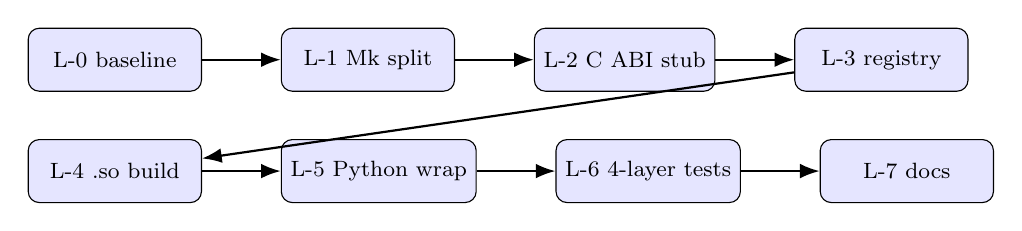
\begin{tikzpicture}[node distance=0.6cm and 1.0cm,
      s/.style={rectangle,draw,rounded corners,minimum width=2.2cm,
                minimum height=0.8cm,align=center,font=\footnotesize,fill=blue!10},
      arr/.style={-{Latex[length=2.5mm]},thick}]
  \node[s] (l0) {L-0 baseline};
  \node[s,right=of l0] (l1) {L-1 Mk split};
  \node[s,right=of l1] (l2) {L-2 C ABI stub};
  \node[s,right=of l2] (l3) {L-3 registry};
  \node[s,below=of l0] (l4) {L-4 .so build};
  \node[s,right=of l4] (l5) {L-5 Python wrap};
  \node[s,right=of l5] (l6) {L-6 4-layer tests};
  \node[s,right=of l6] (l7) {L-7 docs};
  \draw[arr] (l0) -- (l1);
  \draw[arr] (l1) -- (l2);
  \draw[arr] (l2) -- (l3);
  \draw[arr] (l3) -- (l4);
  \draw[arr] (l4) -- (l5);
  \draw[arr] (l5) -- (l6);
  \draw[arr] (l6) -- (l7);
\end{tikzpicture}
\end{center}

% ======================================================================
\chapter*{編集後記}
\addcontentsline{toc}{chapter}{編集後記}

本書は 2026 年 4 月 18 日の集中開発(Phase L-0 〜 L-7)の成果を,
\textbf{初学者が一人で読み進められるように}整えたマニュアルである.
共有ライブラリや ctypes の話は一般に難解な分野だが, 「なぜそうするか」
を丁寧に説明することで, 物理屋の読者が\textbf{自分のスクリプト}を
数分で書き始められる状態を目指した.

ご意見・誤記の指摘は k-yoshimi@g.ecc.u-tokyo.ac.jp まで.

\vfill
\begin{center}\small
TASK プラズマ輸送ライブラリ化プロジェクト --- 日本語マニュアル\\
(tr / ti / wr / wrx / fp, Phase L-0 〜 L-7)\\
© 2026 k-yoshimi. TASK コードの license に準じる.
\end{center}

\end{document}
